\section{Introduction}

This is the introduction. Here's a text citation of \citet{OliveiraJr2015}
and a another version that is sometimes used \citep{OliveiraJr2015}.
The rest is gibberish text.




%%%%%%%%%%%%%%%%%%%%%%%%%%%%%%%%%%%%%%%%%%%%%%%%%%%%%%%%%%%%%%%%%%%%%%%%%%%%%%%
\section{Methodology}

Our algorithm for estimating the source's positioning based on Euler deconvolution revealed that stronger sources may influence the estimated positions of nearby weaker ones. Therefore, it becomes imperative to consider the interplay among magnetic sources to accurately estimate their magnetic parameters and position. Understanding how these magnetic sources interact with each other is crucial for refining our estimation process and ensuring robust results in magnetic parameter estimation.


\subsection{Magnetic inversion: interfering sources}
    
In this study, our objective is to explore three distinct methods for handling interfering sources during inversion. The first approach involves employing the interactive Euler deconvolution method, where interference from other sources is systematically removed in each window. The second method considers interference using the $b_z$ vector. The inversion is performed on the entire set of particles. Lastly, we explore a similar approach as the second method, but applied to the first derivative of $b_z$.


\subsubsection{Iteractive Euler deconvolution}

Our algorithm for estimating the source's positioning based on Euler deconvolution revealed that stronger sources may influence the estimated positions of nearby weaker ones. To address this, we propose a refined algorithm with the following steps:

\begin{enumerate}
  \item \textbf{Automatic Source Detection:} Utilizing blob detection on the total gradient amplitude (TGA), the algorithm segregates sources in descending order of magnitude. This enables the application of Euler deconvolution to obtain an initial position estimation.
  
  \item \textbf{Calculation of Theoretical Magnetic Signals:} The theoretical magnetic signals associated with these sources are computed using a simple dipolar forward model.
  
  \item \textbf{Signal Removal:} The magnetic signal attributed to the strongest source is then removed from the original dataset.
  
  \item \textbf{Enhanced Estimation:} The refined dataset is subsequently employed for the analysis of weaker magnetic sources, leading to an improved positioning estimation compared to the previous step.
\end{enumerate}

This step-by-step procedure is designed to mitigate the impact of stronger sources, thereby enhancing the precision of subsequent inversion analyses.



\subsubsection{Vertical component magnetic field}
A way to improve the inversion results is to perform the magnetic moment estimation of all L sources identified at the same time: 

\begin{equation}
\footnotesize
\label{eq_dipole_bz_all}
\dfrac{\mu_0}{4\pi}
{\begin{bmatrix}
\dfrac{\partial^2}{\partial z \partial x} \dfrac{1}{r_{1,1}}
& \dfrac{\partial^2}{\partial z \partial y} \dfrac{1}{r_{1,1}}
& \dfrac{\partial^2}{\partial z \partial z} \dfrac{1}{r_{1,1}}
& \hdots
& \dfrac{\partial^2}{\partial z \partial x} \dfrac{1}{r_{1,L}}
& \dfrac{\partial^2}{\partial z \partial y} \dfrac{1}{r_{1,L}}
& \dfrac{\partial^2}{\partial z \partial z} \dfrac{1}{r_{1,L}} \\
\\

& 
& 
& \vdots
& 
& 
&  \\
\\
\dfrac{\partial^2}{\partial z \partial x} \dfrac{1}{r_{N,1}}
& \dfrac{\partial^2}{\partial z \partial y} \dfrac{1}{r_{N,1}}
& \dfrac{\partial^2}{\partial z \partial z} \dfrac{1}{r_{N,1}}
& \hdots
& \dfrac{\partial^2}{\partial z \partial x} \dfrac{1}{r_{N,L}}
& \dfrac{\partial^2}{\partial z \partial y} \dfrac{1}{r_{N,L}}
& \dfrac{\partial^2}{\partial z \partial z} \dfrac{1}{r_{N,L}} \\
\end{bmatrix}}_{N x L}
{\begin{bmatrix}
{m_x}_1 \\ {m_y}_1 \\ {m_z}_1 \\ \vdots \\{m_x}_L \\ {m_y}_L \\ {m_z}_L \\
\end{bmatrix}}_{L x 1}
=
{\begin{bmatrix}
{bz}_1 \\ {bz}_2 \\ {bz}_3 \\ \vdots \\{bz}_N 
\end{bmatrix}}_{N x 1}.
\end{equation} \bigskip

In which $r_{i,j} = \sqrt{(x_i - {x_c}_j)^2 + (y_i - {y_c}_j)^2 + (z_i - {z_c}_j)^2}$ is the Cartesian distance between the i-th, $i=1, 2, \hdots N$, observation point $b_z (x_i, y_i, z_i)$ and the j-th, $j=1, 2, \hdots L$, point source $({x_c}_j, {y_c}_j, {z_c}_j)$ and $\mu_0$ is the vacuum magnetic permeability. While the three second-order derivatives in Equation~\ref{eq_dipole_bz_all} are:

\begin{equation}
\footnotesize
\begin{aligned}
\dfrac{\partial^2}{\partial z \partial x} \dfrac{1}{r_{i,j}} &=
\dfrac{3(z_i - {z_c}_j)(x_i - {x_c}_j)}{{r_{i,j}}^5}\ ,
\\
\dfrac{\partial^2}{\partial z \partial y} \dfrac{1}{r_{i,j}} &=
\dfrac{3(z_i - {z_c}_j)(y_i - {y_c}_j)}{{r_{i,j}}^5}\ ,
\\
\dfrac{\partial^2}{\partial z \partial z} \dfrac{1}{r_{i,j}} &=
\dfrac{3(z_i - {z_c}_j)^2}{{r_{i,j}}^5} - \dfrac{1}{{r_{i,j}}^3}\ .
\end{aligned}
\end{equation}   \bigskip

Therefore, taking into account all their mutual signal interference in the N observed data further causes the trade-off between accuracy and running time.




\subsubsection{First derivative of vertical component magnetic field}

The other way to improve the inversion process is by using the first derivative of $b_z$. The latter works  akin to a high-pass filter, thus, reducing the likelihood of the stronger source's long-wavelength signal causing too much interference with weaker ones. We can use the $\frac{b_z}{\partial z}$ by deriving both sides of Equation~\ref{eq_dipole_bz_all} by $z$:

\begin{equation}
\footnotesize
\label{eq_dipole_bz_z_deriv}
\dfrac{\mu_0}{4\pi}
\scriptsize{\begin{bmatrix}
\dfrac{\partial^2}{\partial z \partial x \partial z} \dfrac{1}{r_{1,1}}
& \dfrac{\partial^2}{\partial z \partial y \partial z} \dfrac{1}{r_{1,1}}
& \dfrac{\partial^2}{\partial z \partial z \partial z} \dfrac{1}{r_{1,1}}
& \hdots
& \dfrac{\partial^2}{\partial z \partial x \partial z} \dfrac{1}{r_{1,L}}
& \dfrac{\partial^2}{\partial z \partial y \partial z} \dfrac{1}{r_{1,L}}
& \dfrac{\partial^2}{\partial z \partial z \partial z} \dfrac{1}{r_{1,L}} \\
\\

& 
& 
& \vdots
& 
& 
&  \\
\\
\dfrac{\partial^2}{\partial z \partial x \partial z} \dfrac{1}{r_{N,1}}
& \dfrac{\partial^2}{\partial z \partial y \partial z} \dfrac{1}{r_{N,1}}
& \dfrac{\partial^2}{\partial z \partial z \partial z} \dfrac{1}{r_{N,1}}
& \hdots
& \dfrac{\partial^2}{\partial z \partial x \partial z} \dfrac{1}{r_{N,L}}
& \dfrac{\partial^2}{\partial z \partial y \partial z} \dfrac{1}{r_{N,L}}
& \dfrac{\partial^2}{\partial z \partial z \partial z} \dfrac{1}{r_{N,L}} \\
\end{bmatrix}}_{N x L}
{\begin{bmatrix}
{m_x}_1 \\ {m_y}_1 \\ {m_z}_1 \\ \vdots \\{m_x}_L \\ {m_y}_L \\ {m_z}_L \\
\end{bmatrix}}_{L x 1}
=
{\begin{bmatrix}
\frac{{bz}_1}{ \partial z} \\ \frac{{bz}_2}{ \partial z} \\ \frac{{bz}_3}{ \partial z} \\ \vdots \\\frac{{bz}_N}{ \partial z}
\end{bmatrix}}_{N x 1}.
\end{equation} \bigskip

Where the three third-order derivatives in Equation~\ref{eq_dipole_bz_z_deriv} are given by

\begin{equation}
\footnotesize
\begin{aligned}
\dfrac{\partial^2}{\partial z \partial x \partial z} \dfrac{1}{r_{i,j}} &=
\dfrac{3(x_i - {x_c}_j)}{{r_{i,j}}^5} - \dfrac{15(x_i - {x_c}_j)(z_i - {z_c}_j)^2}{{r_{i,j}}^7}\ ,
\\
\dfrac{\partial^2}{\partial z \partial y \partial z} \dfrac{1}{r_{i,j}} &=
\dfrac{3(y_i - {y_c}_j)}{{r_{i,j}}^5} - \dfrac{15(y_i - {y_c}_j)(z_i - {z_c}_j)^2}{{r_{i,j}}^7}\ ,
\\
\dfrac{\partial^2}{\partial z \partial z \partial z} \dfrac{1}{r_{i,j}} &=
\dfrac{9(z_i - {z_c}_j)}{{r_{i,j}}^5} - \dfrac{15(z_i - {z_c}_j)^3}{{r_{i,j}}^7}\ .
\end{aligned}
\end{equation}   \bigskip



%%%%%%%%%%%%%%%%%%%%%%%%%%%%%%%%%%%%%%%%%%%%%%%%%%%%%%%%%%%%%%%%%%%%%%%%%%%%%%%
\section{Results}


%\begin{figure}[tb]
%\centering
%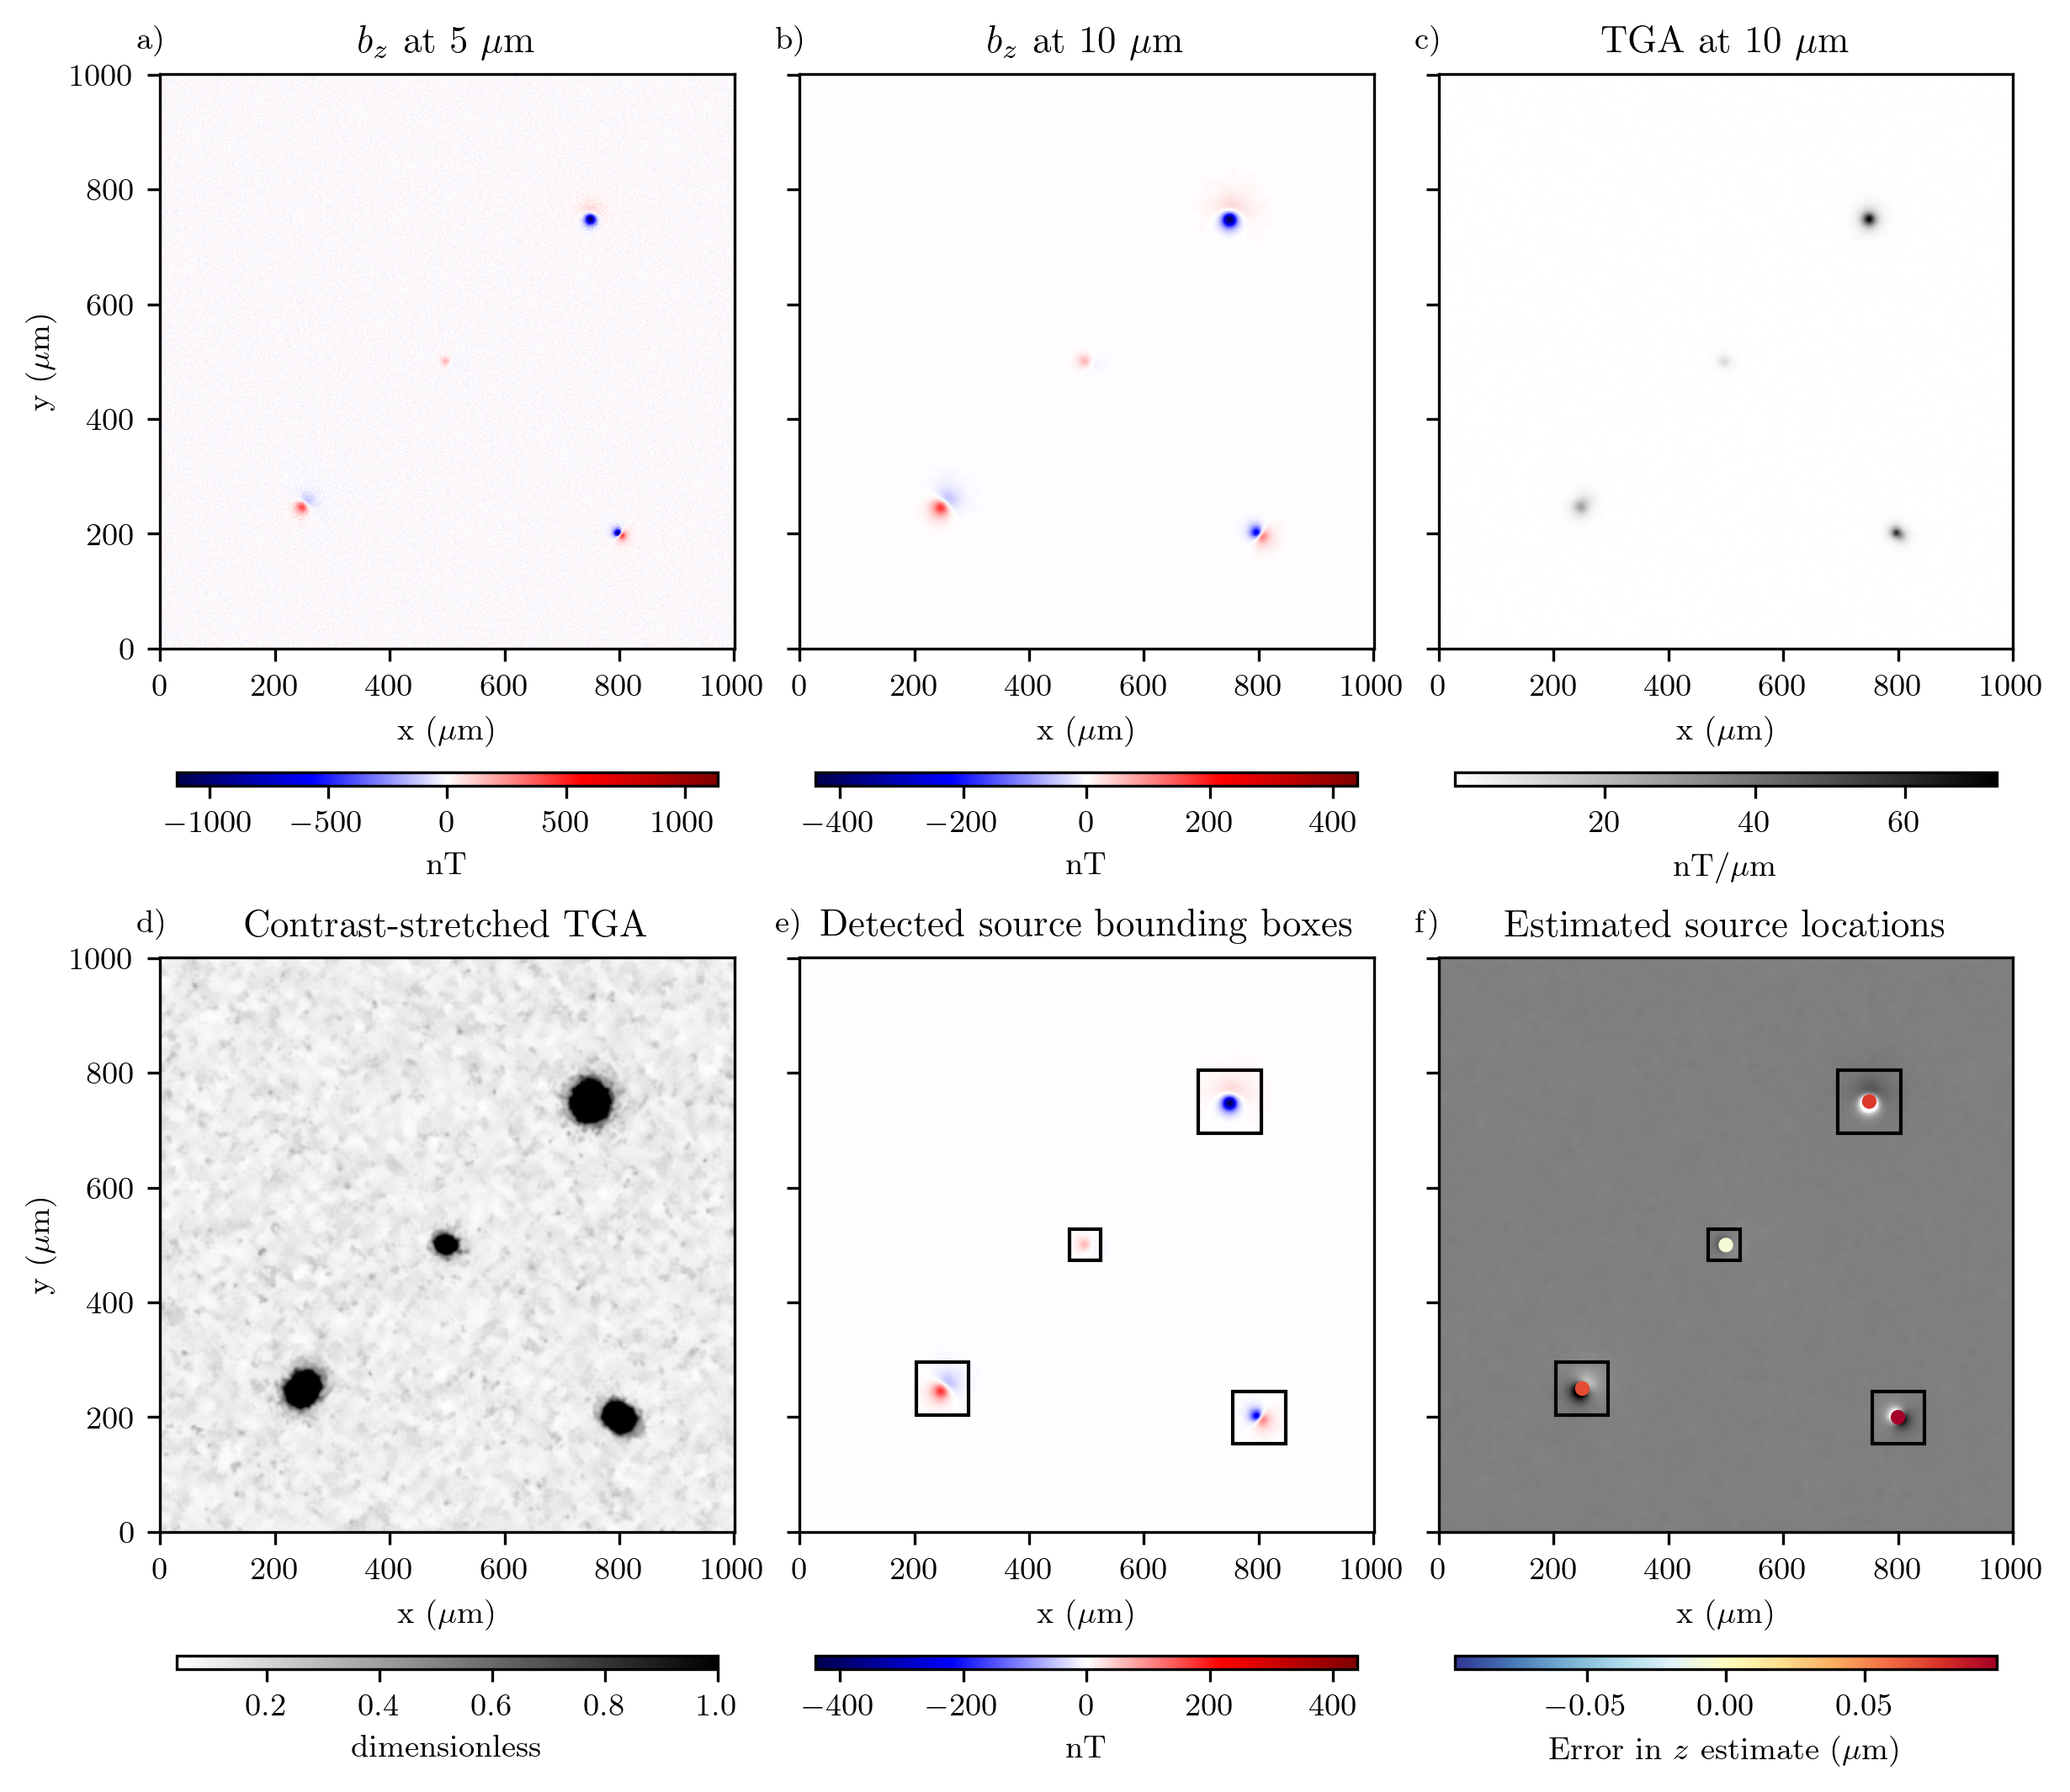
\includegraphics[width=1\linewidth]{figures/simple-synthetic-data.png}
%\caption{
  %\lipsum[1]
%}
%\label{fig_synthetic_simple_data}
%\end{figure}



%%%%%%%%%%%%%%%%%%%%%%%%%%%%%%%%%%%%%%%%%%%%%%%%%%%%%%%%%%%%%%%%%%%%%%%%%%%%%%%
\section{Discussions}


%%%%%%%%%%%%%%%%%%%%%%%%%%%%%%%%%%%%%%%%%%%%%%%%%%%%%%%%%%%%%%%%%%%%%%%%%%%%%%%
\section{Conclusion}



%%%%%%%%%%%%%%%%%%%%%%%%%%%%%%%%%%%%%%%%%%%%%%%%%%%%%%%%%%%%%%%%%%%%%%%%%%%%%%%
\section{Open research}

The Python source code used to produce all results and figures presented here
is available at \url{https://github.com/\GitHubRepository} and
\url{https://doi.org/\ArchiveDOI} under the MIT open-source license.

Here we should cite all of the main software used, like Jupyter, numpy, scipy,
matplotlib, Fatiando, etc.

Cite any data sources as well.



%%%%%%%%%%%%%%%%%%%%%%%%%%%%%%%%%%%%%%%%%%%%%%%%%%%%%%%%%%%%%%%%%%%%%%%%%%%%%%%
\section{Acknowledgements}

We are indebted to the developers and maintainers of the open-source software
without which this work would not have been possible.
Acknowledge any non-author contributors to this study.
Statement about funding.

% Thank the editors and reviewers after review.
